%The Numpy module for Python presents the possibility of using multidimensional arrays. These arrays use dedicated
%structures defined in Numpy for storing metadata. These structures are defined in the Numpy chapter [insert ref].
%The actual memory layout of the data in the ndarrays is described in this subsection. When running Numpy array
%operations on the CELL BE, the memory layout of the arrays becomes critical for performance reasons. The two following subsections
%(red: after the Numpy ndarray structure subsection...rewrite) describes the problems that must be handled and how they can be alleviated.
%Finally, a section shows a small practical example of one way Numpy can be changed to implement a memory layout more suitable for the CELL BE.
%
%The NumPy module for Python is created to implement multidimensional arrays
%for use by Python programmers.  The data in these arrays are managed
%by maintaining meta data in C structures. The most important of these
%structures are presented in section \ref{sec:python-numpy} on
%page \pageref{sec:python-numpy}.
%
This chapter analyzes how the memory layout of NumPy arrays should be,
in order to support an efficient NumPy port to the \CBE{}.

%\subsection{The Numpy ndarray structure}


\section{Finding a Suitable Structure for Cell BE}

When running NumPy on the \CBE{}, the challenge is to employ a good
memory layout, so the following conditions are met:

\begin{itemize}
\item{Data from a single ndarray can be split across multiple SPE's.}
\item{Computations can be done efficiently on the data.}
\end{itemize}

The first condition involves the fact that compute intensive
operations must be done in parallel to be able to utilize the \CBE\
to its full potential.

The latter involves the fact that data must be placed with good
locality, meaning that code running on the SPE's should be able to
fetch data with as few transfers as possible in the general case

In the following, a more thorough analysis of the performance-critical
aspects of the memory layout is given.

\subsection{Two Dimensional Layout to Allow Non-Element-Wise Operations}
\label{sec:fhbdescription}

While many of the operations performed by a Python program using NumPy
arrays might be element-wise operations like matrix addition or
summing, non-element-wise operations must also be supported. An
example of this kind of operation is the level 3 \BLAS\ matrix
multiplication. It's assumed that this kind of multiplication is
performed relatively often in scientific applications, and among other
things it is used when doing blocked LU factorization.

%Imagine doing matrix multiplication in an environment where(//W: hvor vil du hen med dette????)
%\begin{itemize}
%\item{no constraints exists regarding alignment, and}
%\item{the data does not need to be distributed.}
%\end{itemize}

%the operation can be performed with practically no overhead, as long
%as meta data exists telling the program where each row and column
%starts and ends (or this can be computed fast), and strides for the
%dimensions are known.

With the Cell BE architecture, we are dealing with an environment where
both specific alignment and data distribution are required to get a correct and effective implementation.

The figures \ref{fig:1d_layout}, \ref{fig:2d_layout_row_mayor}
and \ref{fig:2d_layout_fhb} illustrates three different memory layouts
of a two dimensional NumPy array. Each layout represents this matrix:

\[ \left( \begin{array}{cccc}
1 & 2 & 3 \\
4 & 5 & 6 \\
7 & 8 & 9 \\
10 & 11 & 12 \end{array} \right)\]

\begin{figure}
\begin{center}
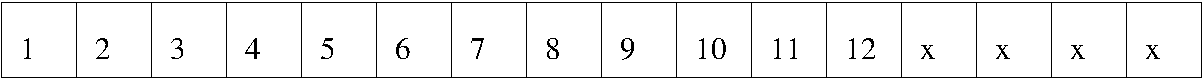
\includegraphics[width=120mm]{./images/1d_layout.pdf}
\end{center}
\caption{One dimensional layout of matrix}
\label{fig:1d_layout}
\end{figure}


\begin{figure}
\begin{center}
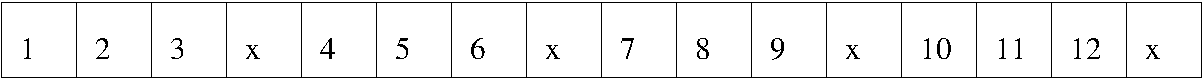
\includegraphics[width=120mm]{./images/2d_layout_row_mayor.pdf}
\end{center}
\caption{Two dimensional layout of matrix in Row Major format}
\label{fig:2d_layout_row_mayor}
\end{figure}

\begin{figure}
\begin{center}
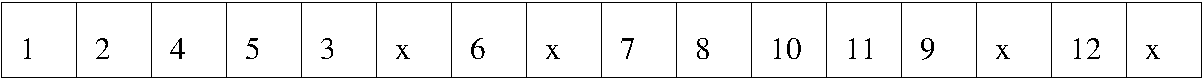
\includegraphics[width=120mm]{./images/2d_layout_fhb.pdf}
\end{center}
\caption{Two dimensional layout of matrix in FHB, Row-Major format}
\label{fig:2d_layout_fhb}
\end{figure}

Each number in the matrix takes up 4 bytes and a 16 byte alignment of
data is needed. Padding is written as \emph{x}'s.

%\begin{figure}
%\begin{center}
%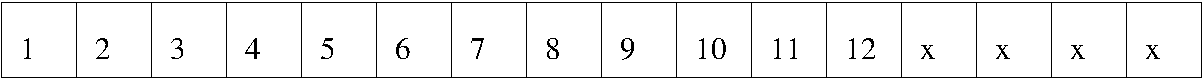
\includegraphics[width=120mm]{./images/1d_layout.pdf}
%\end{center}
%\caption{1d layout of matrix}
%\label{fig:1d_layout}
%\end{figure}


%\begin{figure}
%\begin{center}
%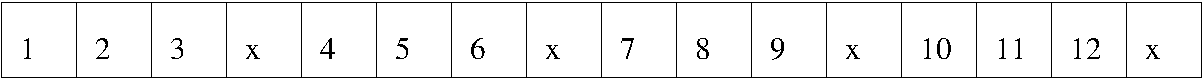
\includegraphics[width=120mm]{./images/2d_layout_row_mayor.pdf}
%\end{center}
%\caption{2d layout of matrix in Row Mayor format}
%\label{fig:2d_layout_row_mayor}
%\end{figure}

%\begin{figure}
%\begin{center}
%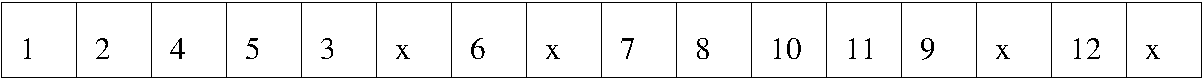
\includegraphics[width=120mm]{./images/2d_layout_fhb.pdf}
%\end{center}
%\caption{2d layout of matrix in FHB, Row-Mayor format}
%\label{fig:2d_layout_fhb}
%\end{figure}

In the layout shown in fig \ref{fig:2d_layout_fhb} a block size of 16
bytes is used for the \FHB\ layout.

When considering how an SPE would operate with these three memory layouts, let's look at each layout in turn, and describe some relevant features.

The order in which each layout is mentioned is intentional. For each new layout mentioned, it is implied that it can also be used as effectively
as the previous mentioned layouts.

\paragraph{One Dimensional Layout}
A one dimensional layout will effectively support all operations that are done element-wise.

\paragraph{Two Dimensional Layout With Row-Major}
This layout will make it possible to easily transfer separate rows to SPE's, since each row is stored aligned in the memory.
However, if a row is larger than what is accepted by a single SPE, additional computations are needed to remedy the situation.
(This can also be said for column major and in either case we might have a situation where neither a single row or a single column
fits into available space in an SPE's \texttt{LS}.)

\paragraph{Two Dimensional Layout With FHB}

The \FHB\ layout makes it possible to arrange data in a way, that
transfers are always easy to do, since each block is stored aligned in
memory and each part of a row in a single block is stored aligned in
memory. The dimensions of a single block can be chosen, so a data
block can always be made to fit in the \LS{}. Because of the structure
of the FHB format, it is also quite easy to index elements and find
which block a given element resides in. Of course, time must be spend
to convert data to the FHB format if the starting point is a
contiguous NumPy array, but when lots of computations are done on the
structure afterwards, the time spend on conversion is negligible. The
FHB format is preferred to the other two, since it allows for
non-element wise operations (like matrix multiplication), without the
need to waste processor time doing computations to locate data and
wasting memory bandwidth to transfer irrelevant data. As an example of
this problem, consider what would happen, if the one dimensional
layout were used to do matrix multiplication on the SPE's. In this
example we have to deal with the following issues:

\begin{itemize}
\item{Data alignment may not fit with the current row length.}
\item{It's somewhat harder to index elements in the array.}
\item{When doing matrix multiplications, each chunk of data on the individual SPE's may not
have an efficient structure.}
\end{itemize}

The FHB layout is described in \cite{scipy}, \cite{hp_storage_hybrid}
and \cite{blockhybridformat}. In these works, the structure is noted
for being effective for level 3 \BLAS\ routines such as matrix
multiplication, because of the blocked structure that gives better
data locality. An important aspect, is that the block size can be
chosen, so a block fits into the LS. The two
articles \cite{hp_storage_hybrid} and \cite{blockhybridformat} states
that the data locality obtained, using a blocked format, efficiently
makes use of the caching hierarchy on a regular machines. In the
context of this thesis and working with the Cell BE, the LS can be
compared to a large level 1 cache of a regular processor.

\section{The ndarray in NumPy}

The ndarray in NumPy is the single most important thing that NumPy
presents to the user. The ndarray is used to represent
multidimensional arrays and matrices. The rest of NumPy basicly
presents the user with ways of manipulating these arrays.

What is interesting, is to determine how the ndarray could be used on
the Cell BE and what modifications would be necessary to make on the
data layout and functions operating on the data layout.

It's assumed that \BLAS\ operations are extensively used in scientific applications, so they must be supported
efficiently for the ndarray on the Cell BE.

It must be decided if operations on ndarrays of more than two
dimensions should be carried out on the SPE's. Specifying element-wise
operations, the abstraction of extra dimensions is not important, but
if non-element wise operations are defined for ndarrays of more than
two dimensions, the data layout of each block in the FHB format
matters.


\subsection{Maximum Two Dimensional Array Operations on SPE's}

Several operations exist in NumPy that allows operations on arrays
larger than two dimensions. These include routines like addition,
multiplication and array-manipulation operations like view creation
and slicing. When doing operations on the SPE's, it becomes a big
issue how many dimensions there may be operated on. The general
assumption is, that NumPy is used for scientific computations. We find
it reasonable to assume that the larger part of a programs execution
time is spend on computation heavy operations involving arrays of
maximum two dimensions. This assumption is based, partly on the fact
that the arithmetic operations defined in the \BLAS\ library definition
involves no function arguments of more than two dimensions
(matrices). It's also assumed that the operations defined in the \BLAS\
definition are used extensively in typical scientific
applications. Scientific applications will therefore benefit greatly
from the possibility of running operations on no larger than
two-dimensional NumPy arrays in parallel on the SPE's. Operations like
view creation and slicing can be supported on the PPE.

Because no more than two dimensions are needed on the SPE's, a basic
requirement is that the FHB format must be used to represent vectors
and matrices. Scalars can be represented as a special case of vectors.

\section{The Data Format Selected For NumPyCBE}

The FHB layout seems like the best general choice, since it allows for
efficient non-element wise operations and can handle alignment issues.

NumPy's \emph{PyArrayObject} structure can be modified to contain meta
data to support the FHB layout. This meta data should include
pointers to all data blocks and data sizes. Furthermore, it might
prove advantageous to have additional information regarding whether a
specific block resides on a specific SPE. In this way, a DMA transfer
could be saved, if the data were found to already be located in
relevant \LS{}'s.

See section \ref{sec:extending_numpy} on
page \pageref{sec:extending_numpy} for a description of how meta data
is stored in NumPy to support the FHB format.

Data blocks in the FHB format must be squares of equal sizes.
This supports operations like level 3 \BLAS\ multiplication well.
Padding is inserted when needed to make the blocks square. 

\subsection{Storing Vectors}
\label{sec:store_vectors}

When using the FHB format to store vectors on the SPE's, it is
advantageous to make a distinction from the way matrices are
stored. If a new vector is created it makes no sense to store parts of
it using only one row of an entire block, leaving the rest of the
block empty. So instead it's chosen to use all space in the blocks to
store vectors.

\subsection{Shortcomings}

A general problem with the FHB layout is that it takes time convert
data to the format. In general, data conversions should be avoided as
much as possible.

Even though it's assumed that maximum two dimensional arrays are used
on the SPE's, there is an issue regarding performance if a matrix is
sliced from an ndarray of higher dimension. As an example, if a three
dimensional array is being sliced into a number of two dimensional
arrays and this slice is done on the "wrong" axis, a considerable
amount of clock cycles might be wasted by the PPE in order to
rearrange data. Figure \ref{fig:fhbslice} represents a bad and a good
slice. The first slice, A, makes a matrix across the third dimension, which
is clearly bad, since data must be rearranged to represent the slice in the FHB format.
The second slice, B, makes a slice, where the data
is already layed out correctly in memory.

\figscale{figures/fhb_two.pdf}{An example of a bad and good slice.}{fig:fhbslice}{0.6}


%\section{Additional rationale behind choosing FHB- REWRITE!!! and maybe move to conclusions?}

%When work began on this report, it was largely motivated by the master
%thesis \cite{scipy}. In this thesis an important conclusion
%is reached about the performance of IBM's BLAS routines optimized for
%the Cell BE. It is mentioned that IBM BLAS does not outperform an
%ATLAS implementation, even when the ATLAS routines only run on the
%PPE. We took this as a sign, that the data structure we should choose
%for porting NumPy's ndarray to Cell BE, must in itself support the
%splitting of data into easy manageable sub problems (e.g. a matrix A
%must be stored in memory, so that data can be split among SPE's
%without having to rearrange data first). Also, since IBM BLAS
%apparently did not perform well, we early on decided that we would
%have to implement our own BLAS routines, that would then perform very
%well with the FHB data layout, at least compared to the ATLAS and IBM
%BLAS results from\cite{scipy}.

%As work progressed, we learned that the results stated
%in \cite{scipy}, while being true, are not very useful. It seems that
%the test results from IBM BLAS were done without regard to the fact
%the IBM BLAS needs to run a single time first, to set up on the
%SPE's. After this single initiation, IBM BLAS has proved to be VERY
%effective. In\cite{scipy}, it is stated that IBM BLAS
%performs poorly because of this initial setup-cost. However, it seems
%that it makes no sense to make a test of IBM BLAS, were only initial
%setup-times are recorded. With the results we have seen in working
%with IBM BLAS, it performs very efficiently. So, while nothing wrong
%is stated in \cite{scipy}, it seems to us, that the results are very
%unuseful, and should not have formed the basis of our initial analysis
%for this master thesis.

%Ref til note om startup overhead: side 13 i http://www-01.ibm.com/chips/techlib/techlib.nsf/techdocs/F6DF42E93A55E57400257353006480B2/$file/BLAS_Prog_Guide_API_v3.0.0.3.pdf.

%BLAS1 and BLAS2 routines have shown to be more effective with IBM BLAS than using our FHB structure with our own BLAS implementation,
%and it is not likely that our implementation of BLAS 3 will be much better than IBM BLAS.

%We assume that IBM BLAS level 3 will use more time rearranging data, where the FHB layout makes data available without having to
%rearrange it, but the speed of the IBM BLAS routines themselves will likely be hard to beat.

%Because of this, we might have followed a different path in the report, if we had had more relevant test results. Instead of deciding early on to use FHB and
%custom made BLAS routines, we might have selected another option, like aligning and padding data in the existing ndarray and
%using IBM BLAS routines to operate on it.

%If IBM BLAS are used with non-contiguous data, an overhead must
%expected, under the assumption that the IBM BLAS implementation uses
%DMA lists instead of being able to transfer large contiguous data
%segments\cite{ibmblas_cell}. However, since BLAS 3 is computation
%heavy, this does not seem to be a big problem.

%In fact, it seems very likely that the NumPy ndarray layout should just be allocated on 128 byte boundaries and then be padded per row in
%order to be able to use IBM BLAS 3 routines effectively.
%(hele rationalet bag FHB var netop at IBM BLAS suttede til 1d layout. Dette skyldes sikkert Rasmus' resultater, som dog ikke direkte er beskrevet som
%vaernede udfoert med 1d data layout.)

%One test in \cite{scipy} page 56, shows that the FHB data layout beats IBM BLAS with a factor 32, but when the test setup that was used is taken into
%account, this test and its results are completely useless.

%\section{Multiplication with FHB}
%//illustrate how multiplication is accomplished with FHB.

%17/04/09 - This section is first attempt at a rewrite
%\section{Datastrucures for Numpy}
%With the assumption that NumPy is being used in a large variety of problem areas, the datalayout
%that is used for NumPy's NDArray must be selected carefully to generally support these areas well.
%It might be worth considering to convert betweeen different datalayouts during execution of a program,
%if this would speed up parts of the program execution time and the time to convert the data is deemed
%neglible in this context.

%Many operations used in scientific computing are done element-wise, where pairs of elements with equal indexes
%needs to be processed together, but no other dependencies exist between elements. For these kinds of operations,
%there is no obvious way to improve runningtimes by exploiting data locality (cache-tuning), so no specific demands
%can be deduced regarding an effective datalayout. In other words, it appears that many different datalayout would work
%equally well for these kinds of operations. The most important aspect seems to be, that time must not be waisted transferring
%elements to LS, if these elements not to be included in the operation at all. This places only minor demands on the datalayout.
%An example of af a datalayout that would not be very sufficient is one where lots of padding elements are included, since
%operating on these padding elements makes no sense.
%However, padding is essential for other operations to perform well.

%Other operations have a different kind of data dependency. The most obviou example of these are the
%matrix multiplication. In this operation a single element in the result matrix depends on elements
%from an entire row and collumn, respectively, from the two matrices. This means that care must taken
%selecting a datalyout that allows the data that shares the most dependencies to coexist in the LS.

%Other considerations must also be taken into account. The hardware specifications of the CELL BE puts
%some demands on the datalayout, if computations on it should be effective.

%As mentioned in [ref. to CELL afsnit], the following demands must be taken into account when analysing datalayout:

%\begin{enumerate}
%\item{Data alignment - in general, data must be 16 byte aligned for practical purposes
%(it is possible to transfer on alignments smaller than 16 bytes, but additional demands must be met in these cases).}
%\item{Data padding - padding is a means to ensure that alignment is maintained effectively.}
%\item{DMA transfers - a smaller number of large transfers are more effective than a larger number of small transfers.}
%\item{Cache lines - Cache lines are 128 bytes.}
%\end{enumerate}

%The datalayout for the NDArray should be useful in general cases. This means that no particular assumptions should be made about the input
%data. For instance, the data cannot be assumed to be aligned and in particular, it cannot be assumed that columns or rows in a
%matrix are aligned.


%A datalayout that seems interesting is the full hybrid block layout (from now on referred to as FHB).

%\subsection{FHB}

%Consider the following matrix:
%\[ \left( \begin{array}{cccc}
%1 & 2 & 3 \\
%4 & 5 & 6 \\
%7 & 8 & 9 \\
%10 & 11 & 12 \end{array} \right)\]
%To illustrate the FHB format the following three figures illustrate how this matrix could be layed out in memory.
%Figure \ref{fig:1d_layout} shows a one dimensional layout, with no padding. This layout would be sufficient for
%element-wise operations. Figure \ref{fig:2d_layout_row_mayor} illustrated a layout with padding. This layout makes
%it possible for rows or columns in a matrix to be aligned and thus enabling efficient transfers. An issue that
%must be taken into account with this layout is what to do, if a row of collumn cannot fit into the LS.
%Figure \ref{fig:2d_layout_fhb} illustrates the FHB layout. This layout can be used to split up a matrix into
%blocks that fit into the LS in a way that supports matrix multiplication.

%\subsubsection{Multiplication with FHB}

%\subsection{5-stencil with FHB}
%FHB is also useful for FHB - it might not be the best choice (Toennesen), but
%can still perform really good.

%\subsubsection{Some benchmarks using FHB from background material}
%backing up that FHB is good

%\subsubsection{Reality check - what performance can be expected from FHB with equally optimized versions using FHB and regualar 2d?}
%How should FHB be used and what could be expected?
%What could be expected when taking into account that some of Rasmus's results don't make sense.
%What is needed to use FHB as a general layout - i.e. support from venders etc.
%  - I denne forbindelse sammenskriv med opfordring fra side 207 i Anderson artikel.

%\subsubsection{Conclusion - is FHB a good choice?}
%What can be expected when using FHB and how thouls this thesis be structured because of that?

%\section{Other alternatives}
%A discussion of stuctures and what is best suited. Basicly a shorter recap of previous section.
%If a single structutre should be selected, FHB seems nice, because... even though...
%In practice there are problem: Using a custom layout... missing support...
%Other structures that makes more sense than FHB when taking vendor libraries into consideration? Can 2d layout be used easeliy with vendor libraries... Should this be
%suggested for practical settings? However - we use FHB as the general structure, but keep the points of practical usefullness in mind.. vendors must support FHB...
